\documentclass[9pt]{article}
\usepackage[landscape,margin=0.38in]{geometry}
\usepackage{amsmath,amssymb}
\usepackage{booktabs,tabularx,array}
\usepackage{xcolor}
\usepackage{enumitem}
\usepackage{tikz}
\usetikzlibrary{arrows.meta,positioning,fit,calc,shapes.geometric}

\pagestyle{empty}
\setlength{\parindent}{0pt}
\setlength{\tabcolsep}{3pt}
\renewcommand{\arraystretch}{1.08}
\setlist[itemize]{leftmargin=1.1em,itemsep=1pt,topsep=2pt,parsep=0pt}

\definecolor{bluebox}{HTML}{E8F1FF}
\definecolor{greenbox}{HTML}{EAF7EA}
\definecolor{redbox}{HTML}{FFECEC}
\definecolor{yellowbox}{HTML}{FFF8D8}
\definecolor{graybox}{HTML}{F3F3F3}
\definecolor{lineblue}{HTML}{2F5C99}
\definecolor{darkgreen}{HTML}{166534}
\definecolor{darkred}{HTML}{B91C1C}
\newcommand{\close}{\textcolor{darkgreen}{$+$}}
\newcommand{\far}{\textcolor{darkred}{$-$}}
\newcommand{\maybe}{\textcolor{orange!80!black}{$\pm$}}
\newcommand{\sg}{\operatorname{sg}}
\newcommand{\simfn}{\operatorname{sim}}

\begin{document}
\small
\begin{center}
{\Large \textbf{Code-JEPA for Agentic Code Self-Training}}\quad
{\normalsize hard-negative-sensitive code geometry for reranking, hindsight feedback, and failure-memory exploration}
\end{center}
\vspace{-0.4em}

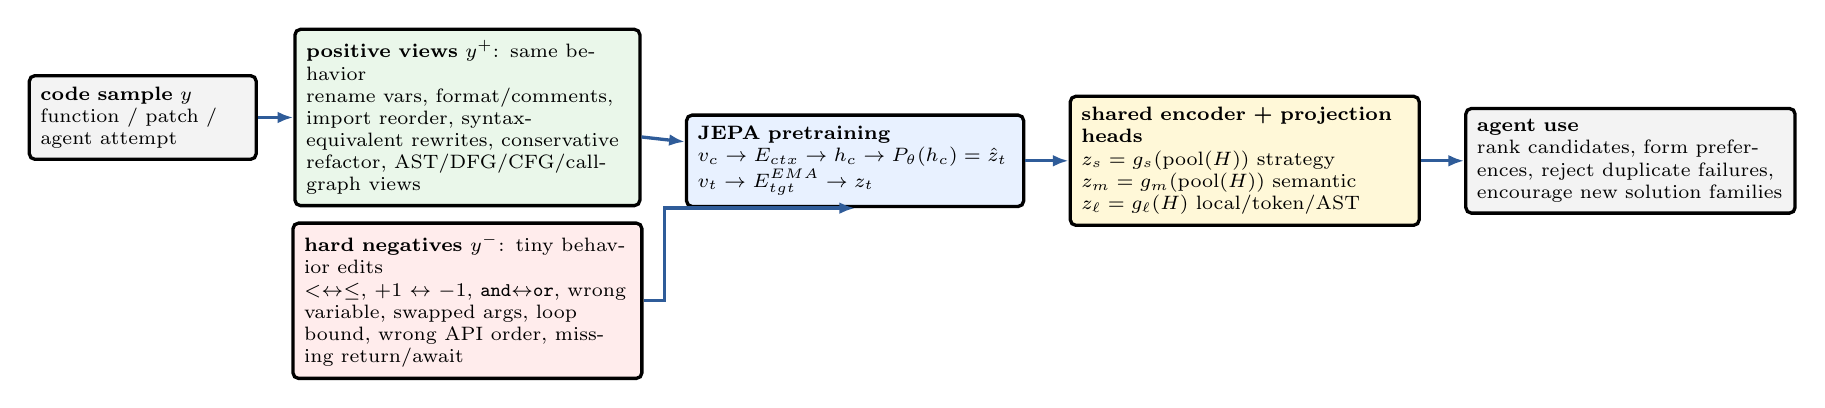
\begin{tikzpicture}[
  font=\scriptsize,
  box/.style={draw, rounded corners=2pt, very thick, align=left, inner sep=4pt, minimum height=0.78cm},
  arrow/.style={-{Latex[length=2mm]}, very thick, lineblue},
  smallbox/.style={draw, rounded corners=2pt, align=left, inner sep=3pt}
]
\node[box, fill=graybox, text width=2.6cm] (code) {\textbf{code sample} $y$\\function / patch / agent attempt};
\node[box, fill=greenbox, text width=4.1cm, right=0.45cm of code] (pos) {\textbf{positive views} $y^+$: same behavior\\rename vars, format/comments, import reorder, syntax-equivalent rewrites, conservative refactor, AST/DFG/CFG/call-graph views};
\node[box, fill=redbox, text width=4.15cm, below=0.18cm of pos] (neg) {\textbf{hard negatives} $y^-$: tiny behavior edits\\$<\leftrightarrow\le$, $+1\leftrightarrow -1$, \texttt{and}$\leftrightarrow$\texttt{or}, wrong variable, swapped args, loop bound, wrong API order, missing return/await};
\node[box, fill=bluebox, text width=4.0cm, right=0.55cm of pos, yshift=-0.55cm] (jepa) {\textbf{JEPA pretraining}\\$v_c \to E_{ctx}\to h_c\to P_\theta(h_c)=\hat z_t$\\$v_t \to E_{tgt}^{EMA}\to z_t$};
\node[box, fill=yellowbox, text width=4.15cm, right=0.55cm of jepa] (heads) {\textbf{shared encoder + projection heads}\\$z_s=g_s(\mathrm{pool}(H))$ strategy\\$z_m=g_m(\mathrm{pool}(H))$ semantic\\$z_\ell=g_\ell(H)$ local/token/AST};
\node[box, fill=graybox, text width=3.9cm, right=0.55cm of heads] (use) {\textbf{agent use}\\rank candidates, form preferences, reject duplicate failures, encourage new solution families};
\draw[arrow] (code) -- (pos);
\draw[arrow] (pos) -- (jepa);
\draw[arrow] (neg.east) -- ++(0.27,0) |- (jepa.south);
\draw[arrow] (jepa) -- (heads);
\draw[arrow] (heads) -- (use);
\end{tikzpicture}

\vspace{0.25em}
\begin{minipage}[t]{0.325\linewidth}
\textbf{1. Training objective}\vspace{0.2em}

Normal JEPA learns predictive latent structure:
\[
\mathcal L_{JEPA}=\|P_\theta(E_{ctx}(v_c))-\sg(E_{tgt}(v_t))\|_2^2.
\]
For code, add invariance and hard-negative geometry:
\[
\mathcal L=\mathcal L_{JEPA}+\lambda_p\mathcal L_{pos}+\lambda_n\mathcal L_{rank}+\lambda_\ell\mathcal L_{local}
\]
\[
\mathcal L_{rank}=\max(0,\,m+\simfn(z(y),z(y^-))-\simfn(z(y),z(y^+))).
\]
Key requirement: harmless rewrites collapse; one-character behavior changes can separate.

\vspace{0.3em}
\textbf{Positive transformations}\vspace{-0.2em}
\begin{itemize}
\item variable/function renaming when safe
\item whitespace, comments, docstrings, quotes
\item import reorder/split/merge when equivalent
\item syntax-equivalent rewrites, conservative inlining/extraction
\item alternate views: AST, DFG, CFG, call graph, dependency graph
\end{itemize}

\textbf{Negative transformations}\vspace{-0.2em}
\begin{itemize}
\item off-by-one, wrong comparator, wrong boolean operator
\item wrong variable, swapped args, wrong default/API order
\item missing edge-case branch, return, exception, await
\item mutate copy vs original, wrong sort direction
\end{itemize}
\end{minipage}\hfill
\begin{minipage}[t]{0.335\linewidth}
\textbf{2. Multi-space similarity}\vspace{0.2em}

Use one expensive transformer backbone, not separate full models. Projection heads define different geometries:
\[
E(y)\to H,\quad z_s=g_s(H),\quad z_m=g_m(H),\quad z_\ell=g_\ell(H).
\]
\begin{center}
\scriptsize
\begin{tabularx}{\linewidth}{>{\raggedright\arraybackslash}Xccc}
\toprule
\textbf{Pair type} & \textbf{strategy} & \textbf{semantic} & \textbf{local} \\
\midrule
format / rename / comments & \close & \close & low \\
behavior-preserving refactor & \close & \close & aligned \\
$<$ vs $\le$, off-by-one & \close & \far & high span \\
wrong variable / swapped args & \close & \far & high span \\
same task, different algorithm & \far & \maybe & diffuse \\
unrelated code & \far & \far & high \\
\bottomrule
\end{tabularx}
\end{center}
\vspace{-0.2em}
\close{} = close, \far{} = far, \maybe{} = close only if both solve the same spec.

\vspace{0.3em}
\textbf{Candidate interpretation}\vspace{-0.2em}
\begin{center}
\scriptsize
\begin{tabularx}{\linewidth}{cc>{\raggedright\arraybackslash}X}
\toprule
$\simfn_s(y_{new},y_{bad})$ & $\simfn_m(y_{new},y_{bad})$ & action \\
\midrule
high & high & duplicate failure / rephrase: reject or deprioritize \\
high & low & same approach but meaningful fix: keep and verify \\
low & any & new solution family: keep for exploration \\
\bottomrule
\end{tabularx}
\end{center}

\vspace{0.2em}
Local vectors prevent the bad failure mode where a global embedding treats
\texttt{i < n} and \texttt{i <= n} as merely ``almost identical''.
\end{minipage}\hfill
\begin{minipage}[t]{0.325\linewidth}
\textbf{3. Downstream self-training loops}\vspace{0.2em}

\textbf{A. Reference-known RLJF.}
Given prompt $x$, reference $y_{ref}$, samples $y_1\ldots y_k$:
\[
score_i=\simfn_m(z_m(y_i),z_m(y_{ref})).
\]
Use top/bottom samples as DPO/RLJF preference pairs; compare against CodeBERTScore/generic embeddings.

\vspace{0.25em}
\textbf{B. Agent eventually succeeds.}
Trajectory $y_1,\ldots,y_T$ with verifier success at $y_T$:
\[
y_{ref}:=y_T.
\]
Use hindsight: attempts closer to $y_T$ become preferred over repeated failures; distill the successful trajectory and train away from earlier failure clusters.

\vspace{0.25em}
\textbf{C. Agent has no solution yet.}
All candidates fail. Store failure memory:
\[
M_{bad}=\{C_j\},\quad C_j=\text{clusters in }(z_s,z_m,z_\ell)\text{ space}.
\]
For new candidate $y$:
\[
S(y)=sanity+fit+\beta\,novelty_s-\gamma\,dup_{bad}.
\]
Reject if it is close to a bad cluster in both strategy and semantic space with no high-impact local change. This rejects rephrasings of known-bad programs; it does \emph{not} certify correctness.

\vspace{0.25em}
\textbf{Safety rule.} Code-JEPA is a geometry/memory/ranking model. Positives require an anchor: reference, tests/verifier, accepted patch, or hindsight success. Pure novelty is exploration only.
\end{minipage}

\end{document}
